% This is "www2010-sample.tex" copied from "www2005-sample.tex" V1.2 January 26 2004
% This file should be compiled with V1.4 of "www2010-submission.class"
%
% This example file demonstrates the use of the 'www2010-submission.cls'
% V1.4 LaTeX2e document class file. It is for those submitting
% articles to the WWW'04 Conference WHO DO NOT WISH TO
% STRICTLY ADHERE TO THE SIGS (PUBS-BOARD-ENDORSED) STYLE.
% The 'www2010-submission.cls' file will produce a similar-looking,
% albeit, 'tighter' paper resulting in, invariably, fewer pages.
%
% ----------------------------------------------------------------------------------------------------------------
% This .tex file (and associated .cls V1.4) produces:
%       1) NO Permission Statement
%       2) WWW'04-specific conference (location) information
%       3) The Copyright Line with ACM data
%       4) NO page numbers
%
% ---------------------------------------------------------------------------------------------------------------
% This .tex source is an example which *does* use
% the .bib file (from which the .bbl file % is produced).
% REMEMBER HOWEVER: After having produced the .bbl file,
% and prior to final submission, you *NEED* to 'insert'
% your .bbl file into your source .tex file so as to provide
% ONE 'self-contained' source file.
%
% ================= IF YOU HAVE QUESTIONS =======================
% Questions regarding the SIGS styles, SIGS policies and
% procedures, Conferences etc. should be sent to
% Julie Goetz (goetz@acm.org) or Adrienne Griscti (griscti@acm.org)
%
% Technical questions only to
% Gerald Murray (murray@acm.org)
% ===============================================================
%
% For tracking purposes - this is V1.2 - January 26 2004
\documentclass{www2010-submission}

\begin{document}
%
\title{Search the Web Using GUI Screenshots}
%\subtitle{[Extended Abstract]
%\titlenote{A full version of this paper is available as
%\textit{Author's Guide to Preparing ACM SIG Proceedings Using
%\LaTeX$2_\epsilon$\ and BibTeX} at
%\texttt{www.acm.org/eaddress.htm}}}
%
% You need the command \numberofauthors to handle the "boxing"
% and alignment of the authors under the title, and to add
% a section for authors number 4 through n.
%
% Up to the first three authors are aligned under the title;
% use the \alignauthor commands below to handle those names
% and affiliations. Add names, affiliations, addresses for
% additional authors as the argument to \additionalauthors;
% these will be set for you without further effort on your
% part as the last section in the body of your article BEFORE
% References or any Appendices.

\numberofauthors{2}
%
% Put no more than the first THREE authors in the \author command

% NOTE: All authors should be on the first page. For instructions
% for more than 3 authors, see:
% http://www.acm.org/sigs/pubs/proceed/sigfaq.htm#a18





\author{
%
% The command \alignauthor (no curly braces needed) should
% precede each author name, affiliation/snail-mail address and
% e-mail address. Additionally, tag each line of
% affiliation/address with \affaddr, and tag the
%% e-mail address with \email.
\alignauthor Tom Yeh, Brandyn White, Larry Davis\\
       \affaddr{University of Maryland}\\
       \affaddr{College Park, MD, USA}\\
       \email{\{tomyeh, brandyn, lsd\}@umd.edu}
%\alignauthor Brandyn White\\
%       \affaddr{Institute for Clarity in Documentation}\\
%       \affaddr{P.O. Box 1212}\\
%       \affaddr{Dublin, Ohio 43017-6221}\\
%       \email{webmaster@marysville-ohio.com}
%\alignauthor Larry S. Davis\\
%       \affaddr{Institute for Clarity in Documentation}\\
%       \affaddr{P.O. Box 1212}\\
%       \affaddr{Dublin, Ohio 43017-6221}\\
%       \email{webmaster@marysville-ohio.com}
\alignauthor Boris Katz\\
       \affaddr{CSAIL}\\
       \affaddr{Cambridge, MA, USA}\\
       \email{boris@mit.edu}
}
%\additionalauthors{Additional authors: John Smith (The Th{\o}rv\"{a}ld Group,
%email: {\texttt{jsmith@affiliation.org}}) and Julius P.~Kumquat
%(The Kumquat Consortium, email: {\texttt{jpkumquat@consortium.net}}).}
%\date{30 July 1999}
%\begin{figure*}[t]
%
\includegraphics[width=2\columnwidth]{authors.png}
%\end{figure*}
\maketitle

\begin{abstract}
Many online articles contain useful know-how knowledge about GUI
applications that are richly illustrated by screenshots.  However, no
system has been designed to take advantage of these screenshots to
visually search this resource effectively.  In this paper, we present a novel
system to index and search software know-how articles that leverages
the visual correspondences between screenshots. To retrieve articles
about an application, users can take a screenshot of the application
to query the system and retrieve a list of articles containing a
matching screenshot.  Useful snippets such as captions, references,
and nearby text are automatically extracted from the retrieved
articles and shown alongside with the thumbnails of the matching
screenshots as excerpts for relevancy judgement. Retrieved articles
are also ranked by a comprehensive set of visual, textual, and site
features, whose weights are learned by RankSVM. Our prototype system
currently contains 150k articles that are classified into walkthrough,
book, gallery, and general categories. We demonstrated the system's
ability to retrieve matching screenshots for a wide variety of
programs, across language boundaries, and provide subjectively more
useful results than keyword-based search web and image search engines.
\end{abstract}

% A category with only the three required fields
\category{H.4.m}{Information Systems}{Miscellaneous}
\category{D.2}{Software}{Software Engineering}
%A category including the fourth, optional field follows...
\category{D.2.8}{Software Engineering}{Metrics}[complexity measures,
performance measures]

\terms{Image search}

\keywords{Image search}

\section{Introduction}

Many online articles contain useful know-how knowledge about GUI
applications. Users can learn from these articles how to perform a
wide variety of tasks, such as how to set up a home network, back up
files, or change the speed of the mouse cursor. These resources are
often created and made available online by software developers who
wish to maintain an online version of the documentation in order to keep the content up-to-date (e.g.,
support.microsoft.com). These resources are also created by
unofficial, third-party experts, for example, by sites offering
tutorials and tips on various software applications (e.g.,
osxfaq.com), by general-purpose \emph{how-to} sites (e.g., eHow.com)
featuring software tutorials as one of the topics, and by computer
book publishers who wish to make their books accessible online via
subscription (e.g., safaribooksonline.com). Even more resources can be
found in user-generated content, for example, in blogs where bloggers
share their experiences and tips using a software application, in
discussion boards where people can discuss and learn from each other
about software, and in QA communities such as Yahoo Answers where
members can raise question and get answers back from other members.

However, for some users, searching this valuable resource
effectively can be challenging. For example, suppose a user opens
up the network properties dialog window and wishes to find out how
to change the IP address. To use a search engine, this user may
first type ``change IP address'' to describe the task he wishes to
learn. He may soon realize it is also necessary to indicate which
dialog window he wishes to perform the task with. To do so, he may
enter additional search terms to describe the operating system,
the title of the dialog window, and any other information needed
to identify the dialog window. Not only is it \textbf{cumbersome
to enter many keywords} but also these keywords are \textbf{prone
to ambiguity} since it is hard distinguish the keywords describing
the program from those describing the task. As the user
browses the links in the result, the user may find it
\textbf{difficult to judge relevancy} based only on the text
excerpts. Moreover, with the emphasis on second language education and the
availability of free and powerful machine translation technology
(e.g., Google Translate),  many Web users have begun to practice
bilingual search in order to access more information beyond the
confine of their native language. However, technical articles are
often \textbf{inaccessible by bilingual search}. For example, a
Chinese-speaking person fluent in English may be able to retrieve
useful articles on dogs in both languages using the English or
Chinese word for \emph{dog} as the search term. But when it comes
to technical terms such as \emph{system preferences}, the same
person may be confined to only Chinese articles since it may not be
obvious how to translate these terms into English.

%(The ranking in this example has been artificially adjusted in
%order to illustrate a rich variety of results.)

\begin{figure*}
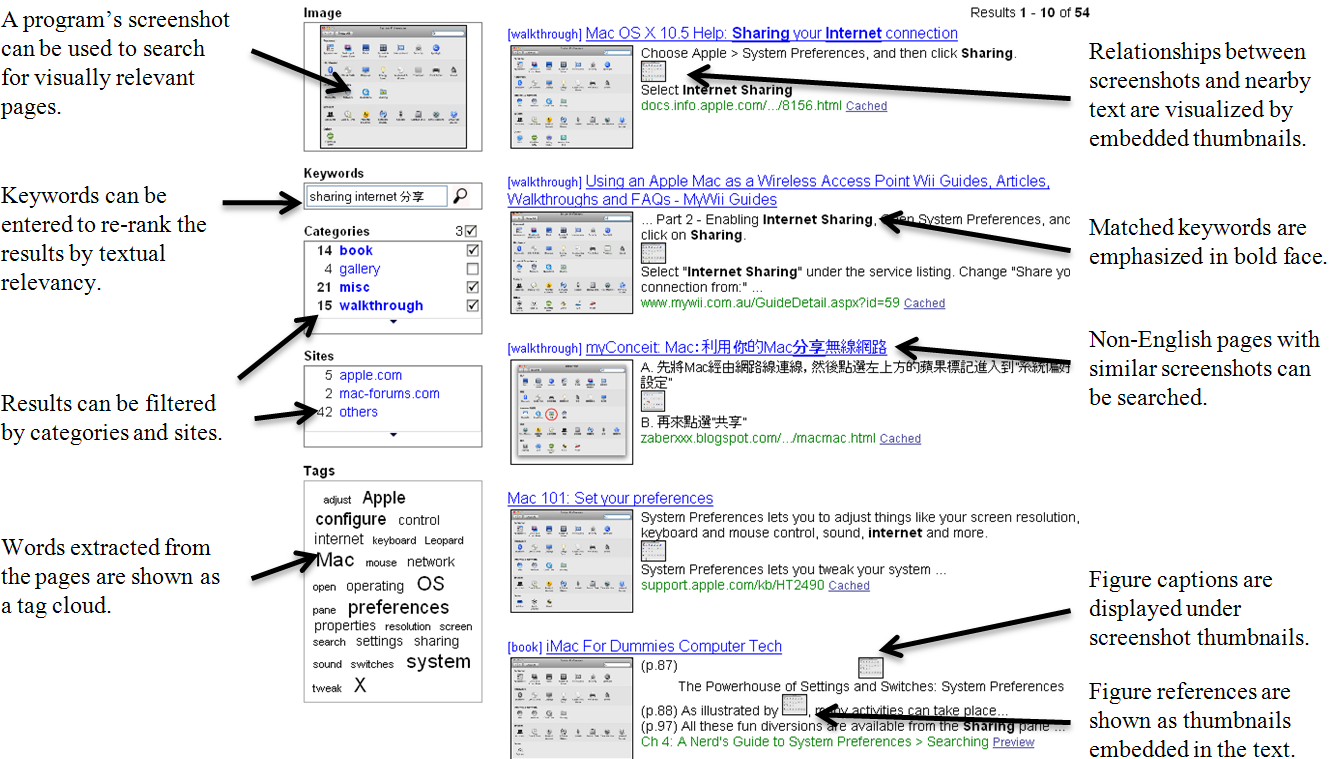
\includegraphics[width=2\columnwidth]{figure/main_result.png}
\caption{A typical result page returned by our
proposd search engine that uses screenshots to search 
for articles about computer programs.}
\label{fig:main_result}
\end{figure*}

In this paper, we present a novel system for indexing and searching
online know-how articles about computer applications (Figure
\ref{fig:main_result}).  These articles tend to be richly illustrated
by screenshots of the applications discussed in the text. Our proposed
system leverages this unique property and adopts a multi-modal
approach to indexing and searching these articles based on both visual
and textual relevance.  It enables computer users to submit a
screenshot of an application as the search term and to retrieve a list
of relevant articles containing the screenshots of the same
application. In addition, it allows users to optionally specify a few
keywords to search within these visually relevant articles for a
subset regarding a specific topic.

Our approach offers several advantages. In terms of usability, this
approach is \textbf{direct and intuitive}. Users only need to capture a
screenshot of an application to form a query, which is less cumbersome
than entering several keywords to describe the application. In terms
of the separation between context and topic, this approach is
\textbf{unambiguous} since each search modality serves a well-defined
role (i.e., context $\rightarrow$ screenshot, topic
$\rightarrow$ keywords). In terms of relevancy judgement, this approach 
is \textbf{cognitively simple}, by reducing the judgement task from
reading text snippets to viewing images.  Finally, in terms of
internalization, this approach is \textbf{language independent} since
it speaks the universal language of images and does not require
users to translate technical terms.

This paper reports on the two major contributions made by the current research:
\begin{itemize}
\item Proposed a multi-modal search engine for computer know-how articles.
\item Built and evaluated a prototype system with more than 150K unique
pages.
\end{itemize}
In the rest of the paper, we review related work (Section
\ref{sec:related_work}), describe the how we built the database for our
proposed system (Section \ref{sec:building}), explain how the database
can be searched (Section \ref{sec:searching}), and describe how the
system was evaluated (Section \ref{sec:evaluation}).

\section{Related Work}
\label{sec:related_work}

There has been a growing research interest in the problem of indexing,
searching, and organizing images on the web.  Many classic problems
originated from text search have been revisited in the new context of
images. For example, Jing and Baluja \cite{Jing} tackled the ranking
problem in the context of searching product images using PageRank.
Kennedy and Naaman \cite{Kennedy} and Van Leuken et al
\cite{vanLeuken} both examined the problem of result diversification in
the context of image search; the former considered a specialized case
of landmark images, whereas the latter considered a more general case
involving a wider range of topics such as animals and cars. Lempel and
Soffer \cite{Lempel} dealt with the problem of authority
identification for web images by analyzing the link structures of the
source pages.  Mehta et al \cite{Mehta} presented a solution to the
problem of spam detection for web images; they analyzed visual
features and looked for duplicate images in suspiciously large
quantities as potential spam.  Li et al \cite{Li} considered the
problem of relevance judgement and demonstrated the ability of image
excerpts (dominant image + snippets) to help users judge results
faster. Crandall et al \cite{Crandall} took on the challenge of
organizing a large dataset in the setting of tens of millions of
geotagged images, taking a comprehensive approach involving visual,
textual, and temporal features. Similar to these existing works, the
current work relies on several state-of-the-art computer algorithms in
order to index and search screenshots effectively. But unlike them,
the current work finds similar images only as an intermediate step
toward the ultimate goal of returning relevant text to the users.

In response to accelerated globalization, there have been research
efforts dedicated to make the Web more accessible to international
users independent of the languages they speak. For example, Scholl et
al \cite{Scholl} proposed a method to search the Web by genres such as
blog and forum in a language independent manner. Ni et al \cite{Ni}
explored ways to analyze and organize Web information written in
different languages by mining multilingual topics from
Wikipedia. Tanaka-Ishii and Nakagawa \cite{Tanaka-Ishii} developed a
tool for language learners to perform multilingual search to find
usage of foreign languages. In relation to research efforts,
the current work offers yet another interesting and promising
possibility---searching based on the universal
visual language of screenshots.

In terms of the application domain, the work closest to ours is that
of Medhi et al \cite{Medhi} who examined the optimal way to present
audio-visual know-how knowledge to novice computer users.  In terms of
search modality, there have been several previous works aimed to
provide users with multiple search modalities instead of just
keywords. For example, Narayan et al \cite{Narayan} developed a
multi-modal mobile interface combining speech and text for accessing
web information through a personalized dialog.  Dowman et al
\cite{Dowman} dealt with the problem of indexing and searching radio
and television news using both speech and text. In the current work,
we explore the potential of the particular modality pair of image and
text for searching computer-related articles.

%Arase et al \cite{Arase} proposed a
%game-based approach to college human assigned relevancy of landmark
%images. Amazon mechanical turk. 

In the current work, we used crowd-sourcing to train and evaluate the
proposed system.  We used the crowd-sourcing serviced brokered by
Amazon Mechanical Turk (AMT), a vibrant micro-task market where people
can be recruited to perform simple tasks for small monetary
awards. AMT has been applied in various research contexts for the
purpose of training and evaluation. Kittur et al \cite{Kittur}
reported success in recruiting workers from AMT to rate Wikipedia
articles and achieved quality comparable to that by expert raters.
Liu et al \cite{Liu} used AMT to evaluate their algorithm for
predicting satisfication of answers in online QA
communities. \cite{Vijayanarasimha} used AMT to label images for
learning visual classifiers.  AMT offers cost-effectiveness and the ability
to cover wider demographics than lab-based studies. However, as
identified by \cite{Kittur}, there are certain risks associated with
this method such as getting dishonest answers, which can be prevented by
formulating the problem in such a way that the optimal strategy for workers is to
perform the task in an honest manner. Thus, in all of our
applications of AMT, we built in validation mechanisms to control
quality.

\section{Building the database}
\label{sec:building}

This section describes the process of building the database for
our proposed search engine.

\subsection{Collecting images}

%With lots of resources like a commercial search companies, it is
%possible to crawl the web and collect a large number of
%screenshots. As an academic research project, we are limited by
%resource. Yet, we still manage to build a research prototype
%database at a non-trivial scale of 100,000 images. These images
%came from three sources.

We used three methods to collect screenshot images to populate our
database. Currently, our prototype system contains more than 150k
images in its index.

First, we submitted computer-related keywords to Bing Images
\footnote{www.bing.com/images} to collect screenshot images of
interactive programs. To increase the likelihood of obtaining the
desired images, we sampled keywords from title bars of the dialog
windows of various computer programs. Some examples of these keywords
are properties, preferences, option, settings, wizard, custom,
installation, network, sound, keyboard ... etc. We turned on the
filter feature to keep only illustrations and graphics, rejecting
obviously non-screenshot images such as images of faces and natural
scenes.  Using this method, we collected approximately 100k images.

Second, we used TinEye\footnote{www.tineye.com}, a reverse image
search engine that can take an image as the query and return a list of
URLs to nearly identical copies of the image found on the Web; it is
designed primarily for copyright infringement detection. We manually
captured screenshot images of more than 300 interactive windows of
popular programs across three of the most popular OS platforms (XP,
Vista, and Mac OS). These images were submitted to TinEye to obtain
about 5,000 images.x

Third, we collected a library of 102 electronic books of popular
software programs. We extracted all the image figures embedded in the
electronic file (i.e., Pdf documents). This method produced about
50k images.

Each method has its own pros and cons. While Bing Image Search
provides the best variety of images, many of them are not visually
relevant to any program at all. TinEye is able to provide visually
relevant images, but these images are ranked only by visual
relevancy; the page containing the highest ranked image may not
necessarily contain any useful information. Computer books are
professionally edited and thus contain the highest quality
text; however, they cover a relatively limited range of applications
and their content isn't as current as compared to the Web. By
using all of these methods, we hope to create a rich repository of
technical information that is both visually and textually relevant
to, and accessible by, general computer users.
 
\subsection{Indexing images}
Our image search task can be categorized as a content-based image
retrieval (CBIR) problem; we are given a screenshot of an application
the user would like information about and the desired result is a
ranked list of visually similar images.  The general CBIR task is
ill-defined as each problem domain imposes requirements on what
aspects of the image are relevant for retrieval.  For example, when
searching for photos of a particular person, we may largely ignore the
scene while focusing on detecting and recognizing faces; however, if
our goal is to collect photos taken at national landmarks, we
would place our focus on the background (for a recent survey on CBIR
methods see \cite{Datta1348248}).

In the domain of common GUI screenshots, we have several desired
properties of a CBIR system.  As book and web screenshots are often
post processed by authors to conserve space and draw attention to
relevant parts of the interface, the image search solution should be
invariant to image manipulations including cropping, scaling,
rotation, color variations, and illumination changes.  Moreover,
visual annotations are commonplace as are compositions of different
screenshots, potentially describing a sequence of user actions.  The
GUI elements themselves often vary visually as interface elements may
be moved, scaled, occluded, and themed.  As a primary goal of the
proposed system is to facilitate cross-lingual search, the proposed
system should handle variations in application text.  Tutorials and
documentation for different software versions are often largely
applicable, though the interface may have new visual elements, an
ideal CBIR system would be robust to minor GUI modifications.  To
serve as a useful method of locating help documentation, the system
must have real-time performance on comprehensive databases of book and
web figures.

Our solution to these problems is to model visually descriptive
regions of the image individually.  This allows for spatial variations
and substantial performance gains as only visually relevant regions
of the image are considered.  The images are converted to gray to
reduce common color theme variations and the differences between gray
and color images often found in PC help books and websites
respectively.  To achieve scale, rotation, and illumination
invariance, we use the SURF feature point detector and descriptor
\cite{VanGool1370556} to find and describe regions of interest.  The
SURF descriptor produces a 64 dimensional feature vector for each
feature point found and, for our purposes, the spatial coordinates and
scale of the features are neglected.

Given a list of feature vectors for each image in our database, our
aim is to produce a fast image comparison system.  A possible solution
is to store all of the feature vectors for all images and, given a
query image, cast a vote for each database image that has a feature
within some Euclidean distance to a query image feature; however, this
method would require a substantial amount of memory to allow for fast
comparison.  Moreover, every query feature would be compared to every
database feature, preventing real-time performance on even modestly
sized databases.  To combat this problem, we use the method described
in \cite{Schmid1478419}.  Provided a database of book and web images,
we compute SURF features. The features are clustered using K-Means,
and each individual feature is assigned to its nearest cluster.  For
each cluster, we compute the median value for each of the 64
dimensions in the SURF descriptor.  For each feature in the cluster,
we compare the cluster's median value to the feature vector, producing
a 64 dimension bit-string encoding each dimension's proximity to the
median value.  This process results in what is referred to as a
Hamming Embedding of the feature vector, which requires 8 bytes of
memory for each feature (compared to 256 bytes for the floating point
vector) and allows for fast distance computation by simply taking the
Hamming distance between two bit-strings belonging to the same
cluster.

The offline database process is implemented using the Hadoop
map/reduce \cite{Ghemaqat1327492} implementation to allow the
computation to scale with the database size.  The entire feature
computation and indexing procedure for our 150,000 image database
takes under two hours on a cluster of six High-CPU Amazon EC2
instances.

\subsection{Extracting Snippets}
\label{sec:extracting_snippets}

After collecting and indexing a large number of screenshots, we need
to extract relevant text from their source articles. The objective of
text extraction is to identify snippets in an article that can
highlight and/or give hints about the kinds of knowledge users can
expect to obtain if they read the article. For example, for an article
containing a screenshot of the network configuration program, a good
snippet would be ``set IP address'' or ``enable wireless network''
since it clearly indicates to users the article is likely to explain
how to perform these tasks. On the other hand, a snippet such as
``network configuration'' that describes the screenshot's content is
less useful to users since they already see the content in the
screenshot and learn nothing new from reading the content again in the
snippet. Note that this is in sharp contrast with typical image search
engines that actually favor snippets describing image contents in
order to index and search images. Below we describe six kinds of
informative snippets that we extract for the purpose of our search
application:

\begin{description}

\item[Title/Heading] An article's title and headings are 
  obvious choices for snippets since they often highlight the most
  important points covered by the article. Titles can be extracted
  from the <title> tag for web pages. Headings are especially useful
  when there are multiple screenshots contained in the same
  article. For web articles, we extract the heading tag (e.g., h1, h2)
  closest to and proceeding each screenshot. For book articles, we
  extract the chapter and section headings from the outline metadata
  stored in the PDF file whenever such metadata is available.

\item[Alt Text] An image's ALT tag provides information redundancy in
  cases where the image fails to be displayed. The text attribute of an
  ALT tag is often a useful feature for a keyword-based image search
  engine to index and search images. Based on our observation, the Alt
  text of the screenshot of a program (e.g., Alt=``system preferences'') tends
  to be the title of the program (e.g., System Preferences).
  Thus, such text may not provide any additional information other
  than what the users can already read directly on their computer
  screen. Yet, we expect Alt text can still be helpful in
  strengthening users' confidence in a search result, by checking
  whether both the program's screenshot and title appear in the
  result's excerpt.

\item[Caption] Many screenshot images are accompanied by caption text
  to briefly describe the idea meant to be illustrated by the images.
  Especially in books, almost all the figures, whether or not they are
  screenshots, contain captions that can reliably extracted by looking
  for string patterns that begin with the word Figure.  Even in the
  articles on the web, captions can sometimes be found below or above
  images. These captions are harder to detect because often they are
  not explicitly labeled by the word Figure. Thus, we identify
  potential caption text based on two simple heuristics: (1) is it
  immediately above or below the image and (2) does it have a
  different style as compared to surrounding paragraphs.

\item[References] Sometimes references to images can be found in
  sentences relatively far away from the images. Some references are based
  on explicit labels, such as the phrase \emph{as shown in Figure
    X}. Other references are based on layout relationships, such as 
  the phrase \emph{see below}. Sentences containing such
  references are likely to be relevant to the images they refer
  to. Presented in the excerpt, these sentences may indicate the types
  of knowledge users can expect to learn if they read the whole
  article. To resolve a label-based reference, we look for the image
  whose caption contains the matching label. For web articles, the
  image is always on the same page, whereas in book articles, the
  referred image can appear a few pages away due to formatting
  limitations. To resolve a layout-based reference, we scan in the
  direction indicated in the reference (e.g., scan backward for see
  below) until an image is found. After resolving the reference, a
  link between the referred image and the referring sentence is
  established. Whenever an image is retrieved, sentences referring to
  it can also be retrieved for inclusion in the excerpt.

\item[Action Phrases] Since one of the anticipated uses of our system
  is to learn how to perform interactive actions using a particular
  program, phrases containing certain action keywords can
  be useful. For examples, phrases containing keywords such as
  configure, click, and open, may indicate to the users that the
  article are likely to explain what can be configured, what should be
  clicked, and what must be opened, using the program. Thus, we
  compile a list of common action keywords and extract action phrases
  from each images' surrounding text.

\item[Nearby Text] If none of the above useful excerpt phrases can be
  extracted, we simply extract nearby sentences around the image and
  use it as the excerpt.

%% \item[Figure OCR] Useful text are those the user does not already
%% know. Text that can also be found in the figure is not as useful.
%% Thus, we apply OCR on each figure to determine what text is
%% already embedded in each figure. While these OCR text might not be
%% that useful to the users, since they can already read them, such
%% text can be useful for filtering out sentences that are simply
%% repeat of what is in the figure and thus less useful to the users.

\end{description}

\subsection{Classifying articles into categories}

In addition to extracting useful text from articles, we can also
classify them into distinct categories based on their origins,
structures, and contents.  In the current work, we consider four
categories: book, walkthrough, gallery, and general. The book category
consists of those articles extracted from pdf books. The walkthrough
category includes articles giving step-by-step instructions on how to
perform certain computing tasks such as backing up files and changing
display resolution. Figure \ref{fig:example_walkthrough} shows some
examples of walkthrough articles. These walkthrough articles tend to
possess three features that can help us identify them. First, they
tend to contain an ordered or unordered list of instructions in short
sentences interspersed with screenshot illustrations.  Second, these
sentences tend to begin with common interactive action verbs such as
click, enter, type, and open. Third, walkthrough articles tend to
include certain indicative terms such as walkthrough,
step, and guide. The gallery category consists of articles with many
images but relative small amount of text. The general category covers
all of the unclassified articles. Table \ref{tbl:category_distribution}
summarizes the distribution of articles over the categories.

\begin{figure}
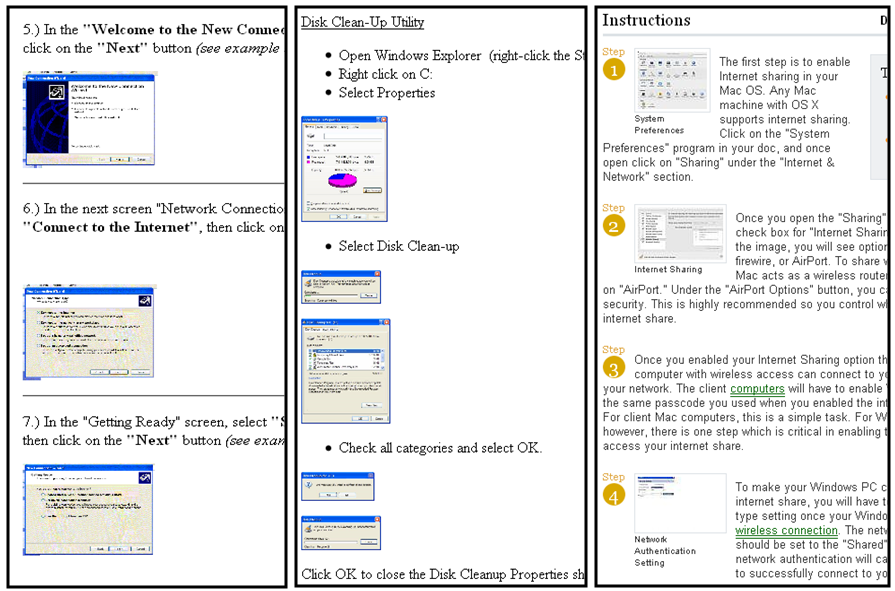
\includegraphics[width=1\columnwidth]{figure/walkthrough_examples.png}
\caption{Examples of articles providing step-by-step walkthroughs.}
\label{fig:example_walkthrough}
\end{figure}

\begin{table}
\centering \caption{Number of articles in each category.}
\label{tbl:category_distribution}

\begin{tabular}{|c|c|c|c||c|}
\hline
  % after \\: \hline or \cline{col1-col2} \cline{col3-col4} ...
      General & Walkthrough & Gallery & Book & Total\\
\hline
 51,743 & 45,249 & 4,464 & 55,244 & 156,700\\
 
 (33.1\%) & (28.9\%) & (2.9\%) & (35.1\%) & \\
\hline
\end{tabular}

\end{table}

%\subsection{Statistics}

%What are the websites hosting the most number of screenshots?

%What are the types of websites hosting useful screenshots?


\section{Searching the database}
\label{sec:searching}

This section describes the process of searching the database. This
process involves specifying queries (Section
\ref{sec:specifying_queries}), 
retrieving articles with similar
images (Section \ref{sec:finding_similar_images}), ranking retrieved
articles
(Section \ref{sec:ranking_retrieved_articles}), and presenting them to
the users
(Section \ref{sec:presenting_results}).

\subsection{Specifying queries}
\label{sec:specifying_queries}

Our proposed search engine supports mixed-modality queries in order to
optimize the effectiveness in searching technical articles about
interactive programs. A typical query consists of a screenshot of a
program and, optionally, a set of keywords to specify what aspects of
the program the retrieved articles are supposed to cover.

Screenshot queries can be specified in two ways. First, users can
run a cross-platform, Java-based, client interface we developed to
capture the screenshot of a selected window or an arbitrary screen
region. The client interface will submit the screenshot as the
image query to our search engine and display the search results in the
default web browser. Alternatively, users can use any existing
image capture utilities such as the snipping tool on Windows Vista
or the Command-Shift+4 hotkey on Mac OS to capture screenshots.
Users can use a Web interface to submit the screenshots to Sikuli
Search and view the results directly.

Keywords queries are optional and can be specified in three ways.
They can be entered together with the screenshot queries on both
the client and Web interfaces. Also, as the users are browsing the
results, they can enter keywords to filter and/or refine the
results.

\subsection{Finding similar images}
\label{sec:finding_similar_images}

Given a query screenshot, we need to find other similar screenshots in
the database in order to retrieve visually relavent articles.  To do
so, we extract visual features from the query image and compute the Hamming
Embedding for each feature as was performed on the database images.
The distance between each query bit-string is computed against all
database bit-strings in the nearest cluster to the query feature
vector.  All features within a certain Hamming distance cast a vote
for their corresponding database image.  This look-up process uses an
inverted file for each cluster which contains lines of bit-strings and
their corresponding database image IDs.  The result is a histogram of
image votes from which we produce a ranked list of database images as
compared to the query image. The average retrieval time for a query
image when $k=1,000$, where $k$ is the number of clusters, is .53
seconds on a single CPU 2.4GHz machine.

\subsection{Ranking retrieved articles}
\label{sec:ranking_retrieved_articles}

After retrieving a list of articles ranked by visual similarity, we
need to re-rank them by taking textual relevancy into account.  If
ranking is based only on visual similarity, as in the case of a
typical content-based image search engine, even though the highest
ranked article may contain the right screenshot, there is no guarantee
whether the article also contains any useful text. Similarly, if
ranking is based only on text, as in the case of a typical keyword
search engine, despite having all the keywords, an article may still
be useless if it contains the wrong screenshot. Therefore, it is
necessary to adopt a ranking scheme based on a comprehensive set of
multimodal features. In the current work, we consider three types of
features: visual, text, and site, which will be explained in detail
next.

\subsubsection{Visual Features}

\begin{description}

\item[Similarity] In our system, visual similarity is the most
  dominant feature. To users, an article with a visually dissimilar
  screenshot is a sure sign that the article is about the wrong
  program and should be ranked lower. However, images with lower
  visual similar scores can simply mean they are a cropped version of
  the same image or a version with it superimposed on another
  image. In some cases the users may still find them useful; there is
  no reason to reject them completely. Hence, we derive a visual
  similarity feature by normalizing the the score by the highest score
  in the result set.

\item[Resize ratio] When a screenshot image of a program is captured
  and included in an article, it is often resized to dimensions that
  are most suitable for reading. The ratio by which an image is
  resized provides a cue as to the image's role. For example, an image
  subject to a high resize ratio may suggest that it is displayed as a
  thumbnail to provide just enough details for identification, whereas
  a moderately resized image may suggest the desire to preserve more
  details for users to actually read its content. The resize ratio
  can be computed as the ratio of the captured size (off the desktop
  screen) and the embedded size (in a Web or book page). The captured
  size can be derived simply from the size of the query image. For
  images extracted from PDF books, the size information is often
  readily available. For Web images, the embedded size is often
  contained in the width and height fields of the \texttt{<img>} tag. In the
  absence of these fields, the size can be extracted from the header
  of the image file. We sampled a number of websites with good
  screenshots and computed the average resize ratios as the standard.
  Then, given an arbitrary screenshot, we can calculate a normalized
  score based on how close it is to the standard.

\item[Position] If an image occupies a prominent position in an
  article, it is likely to be important. As a result, the article may
  dedicate more text to the image and should be ranked higher.  We
  consider three positions to be prominent: first, center, and
  last. We can compute three distinct position scores as the
  normalized distances to each of the three prominent positions.

% \item[Number of coexisting images] The fewer unrelated images a page has,
%   the more likely the information on the page will be about the
%   matching image. This count has to exclude images that are not screenshots.

\end{description}

\subsubsection{Text Features}

\begin{description}

\item[Snippet] If an article contains image related snippets such as
  captions, references, and nearby text, it is likely to be more
  relevant to the image. We derive a binary feature for each type of
  snippet to indicate whether the snippet can be identified in the
  article.

\item[Category] When it comes to technical information, articles in
  some categories may be preferred over others and should be ranked
  higher accordingly. Currently, we consider four categories:
  walkthrough, gallery, general, and book, and derive a binary feature
  for each category.

\item[Search terms] If an article contains more search terms, it is
  likely to be more relevant and should be ranked higher. We check
  whether search terms can be found in the title and in each image
  related snippet. Then, we check whether the search terms can be
  found in the same page. The score is computed as the ratio between
  the number of search terms found and the total number of search
  terms. Then, for matched search terms on the page, this score is
  inversely weighted by their distance to the image. Also, each
  term is inversely weighted by its global frequency in order to favor
  less common terms over very common terms.

\end{description}

\subsubsection{Site Features}

\begin{description}

\item[Authority] Some sites may be trusted by users more for their
  technical content. We identified a list of sites users
  may find authoritative, including sites hosted by software vendors
  such as Microsoft and Apple and those dedicated to know-how
  knowledge such as eHow and wikiHow. We derived a
  binary feature for each site.

\item[Quantity] Some sites may contain relatively more screenshots,
  which may suggest their stronger dedication to technical contents
  involving screenshots.  We counted the number of unique screenshots
  collected from each domain and rank all the domains by this
  number. We then used the percentile in the ranking to compute a
  numerical feature between 0 and 1. Table \ref{tbl:top10sites} lists
  the 10 sites in our database that have the most number of images.






%% \item[Quality]

%% If screenshot images hosted by a site have been consistently
%% judged by users to be accompanied by high-quality text, it's more
%% likely new screen images found on this site will also be
%% accompanied by high-quality text. Initially, we do not have any of
%% this information. We assume images on all websites have equal
%% quality. Average ranking score of the site.

\end{description}

\begin{table}
\centering \caption{Top 10 sites with the most images}
\label{tbl:top10sites}
\begin{tabular}{|c|c||c|c|}
\hline
microsoft.com & 320 & qweas.com & 110 \\
ehow.com & 183 & softpedia.com & 110 \\
brothersoft.com & 163 & bestshareware.net & 108 \\
techrepublic.com & 121 & gateway.com & 106 \\
versiontracker & 113  & askdavetaylor.com & 106 \\  
\hline
\end{tabular}
\end{table}


\subsubsection{Setting feature weights}

Since not all features are equally important, it is necessary to set
the weights appropriately in order to reflect these features' relative
importance. In developing the prototype of our system, we set the
weights in three stages. Table \ref{tbl:feature_weights} lists all the
features and indicates the stages when the weights are set. First
(stage 1), we apply RankSVM to learn feature weights based on the
training data collected using Amazon Mechanical Turk. RankSVM was
originally proposed by Joachims \cite{Joachims} to learn how to weight
features from a set of subjective ordering constraints inferred from
user click-through data to improved ranking. At the development stage,
we did not have any click-through data to derive ordering constraints
for RankSVM. Thus, we recruited workers from Amazon Mechanical Turk to
provide us explicit article ratings from which to infer ordering
constraints. We chose five query images known to retrieve a large of
number of articles, but they are ranked only by visual similarity. We
shuffled the order of these articles and presented them in a list,
Each worker was asked to rate each article in terms of usefulness on a
5-point scale. For quality control, we included two junk results and
two duplicate results. To pass the quality test, workers must
successfully mark junk results as useless and give consistent ratings
to duplicate results. Then, each pair of ratings provided us with an
ordering constraint for training RankSVM. Note that since there was no
easy way to ask the workers to provide meaningful keywords, this
procedure only applied to the subset of features that do not depend on
keywords.

Next (stage 2), we set the weights of keyword-related features based
on the weights of corresponding features. For example, if the weight
of \emph{has\_title} feature is high, it is likely the weight of
\emph{has\_keywords\_in\_title} must also be high. Thus, we set the
weight of each keyword-releated feature to 1.5 times the weight of its
corresponding feature learned at the previous stage. Finally (stage
3), with all the weights set at a reasonable level, we can deploy the
system and continue to refine the weights using RankSVM based on
actual user click-through data.


\begin{table}[t]
\centering \caption{Features for ranking retrieved 
articles. Checks
indicate the stages when weights are set. 
Features with highest weights are shown in bold.}
\label{tbl:feature_weights}
\vspace{0.2cm}

\begin{tabular}{|c|l||c|c|c|}
\hline
Type & Name & 1 & 2 & 3 \\
\hline
\hline
Image & \textbf{visually\_similar} & & & $\surd$ \\
& common\_resize\_ratio &$\surd$& & $\surd$\\
& position\_to\_first &$\surd$& & $\surd$\\
& position\_to\_center &$\surd$& & $\surd$\\
& position\_to\_last &$\surd$& & $\surd$ \\
\hline
Text & \textbf{has\_title} &$\surd$& & $\surd$ \\
& has\_caption &$\surd$& & $\surd$ \\
& \textbf{has\_reference}  &$\surd$& & $\surd$\\
& has\_nearby\_text &$\surd$& & $\surd$\\
& \textbf{is\_walkthrough} &$\surd$& & $\surd$\\
& is\_book &$\surd$& & $\surd$\\
& is\_gallery  &$\surd$& & $\surd$\\
& is\_general &$\surd$& & $\surd$\\
& \textbf{has\_keywords\_in\_title}  &&$\surd$ & $\surd$ \\
& has\_keywords\_in\_caption &&$\surd$ & $\surd$ \\
& \textbf{has\_keywords\_in\_reference} &&$\surd$ & $\surd$\\
& \textbf{has\_keywords\_in\_nearby\_text} &&$\surd$ & $\surd$\\
& keywords\_distance\_to\_image && $\surd$ & $\surd$\\
\hline
Site & \textbf{site\_is\_authority} &$\surd$& & $\surd$\\
& site\_has\_many\_images &$\surd$& & $\surd$\\
\hline

\end{tabular}
\end{table}



\subsection{Presenting results}
\label{sec:presenting_results}

%% New presentation scheme is needed for our purpose. In text search,
%% the keywords are highlighted, and displayed in the context of the
%% text before and after them. In image search, only the caption,
%% url, and dimensions are displayed. Users pay attention to images
%% to judge visual relevancy. Also, they pay attention to the url to
%% judge authority. In Tineye search (reverse image search), the
%% matched images are shown as thumbnails, grouped by "exact copies",
%% and ordered by visual similarity. The back links to the pages
%% where matched images are found are also displayed. All these are
%% not suitable for our purpose.

%% \subsubsection{Result}


\begin{figure}
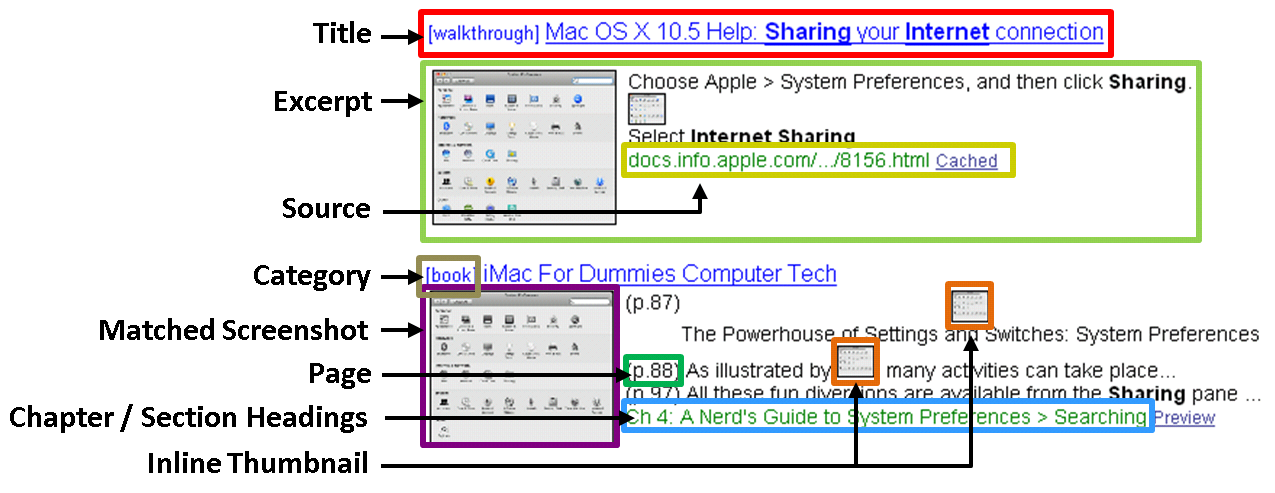
\includegraphics[width=\columnwidth]{figure/result_tile.png}
\caption{Elements of result presentation}
\label{fig:result_tile}
\end{figure}

To display a list of search results, we adopt a presentation scheme 
modeled after that of a typical search engine in order to 
leverage users' existing familiarity with such scheme.  Figure
\ref{fig:result_tile} shows a typical presentation of a single
result. This presentation consists of three main elements: title,
excerpt, and source, that are common for all result types. In addition
there are several minor elements such as tags and actions that
are dependent on the types of results.

For the title element, we display the HTML title tags for web articles
and the book titles for book pages. Markers are inserted
at the beginning of the title to identify the categories (i.e.,
walkthrough, book, or gallery). Users can click on the title to
visit the website to read articles online or preview the content of
the book pages (assuming the copyright issues have been resolved).

For the excerpt element, we display the thumbnail of the matched
screenshot as well as a composition of relevant text snippets
extracted using the methods described in Section
\ref{sec:extracting_snippets}. We insert a tiny inline thumbnail (15
by 15 pixels) into each snippet in a way to reflect the snippet's
type. For a caption snippet, the tiny thumbnail is displayed above the
snippet and centered. For a reference snippet, any explicit figure
label is replaced by the tiny thumbnail of the corresponding
screenshot (i.e., \emph{as shown in Figure 2} $\rightarrow$ \emph{as shown in}

\includegraphics[height=0.2in]{figure/tiny.png}). For a nearby text snippet, the
tiny thumbnail is displayed above or below depending on the image's
relative position. If keywords are specified, their occurrences in the
excerpt are highlighted.

For the source element, we display the abbreviated url for web
results and chapter/section headings for book results.

\subsubsection{Faceted search}

To help users browse search results more effectively, we provide a set
of faceted search capabilities based on the Exhibit framework
developed by Huynh et al \cite{Huynh}. Exhibit is a popular framework for
creating dynamic exhibits of data collections and provides a rich set
of faceted search functionatlies such as filter and timeline
controls. Figure \ref{fig:main_result} shows the two faceted filtering
control displayed at the left-side panel to allow users to filter the results
based on categories and sites.

We also display a tag cloud based on the snippets extracted from all
the retrieved articles. Figure \ref{fig:tag_clouds} shows two examples
of tag clouds.  The size of each tag indicates the number of articles
this tag can be found.  Stop words and words with low article counts
are removed. The tag cloud can help users in three ways. First, it
provides users with a quick overview of the range of topics covered by the
retrieved articles.  Second, the application name also appears in the
cloud as prominent keywords, users can be more confident in the
relevancy of the results. Third, by clicking on a tag, users can
filter the results down to only those containing the tag.

\begin{figure}
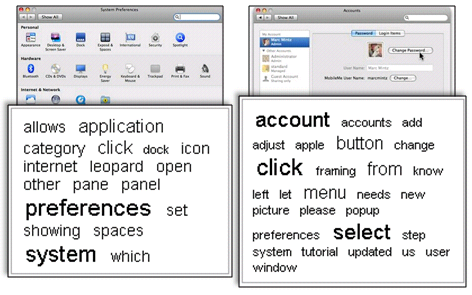
\includegraphics[width=1\columnwidth]{figure/tag_clouds.png}
\caption{Examples of tag clouds generated from the 
results of two screenshot queries.}
\label{fig:tag_clouds}
\end{figure}


\section{Evaluation}
\label{sec:evaluation}

We conducted three sets of experiments to evaluate the proposed system.

\subsection{Screenshot matching performance}

In this experiment, we evaluated the core functionality of our system:
the ability to search for similar screenshot images.  We created a
test set by capturing the screenshots of 352 unique application
windows. This test set covers three major operating systems (Windows
XP, Windows Vista, and Mac OS X) and several popular programs such as
Microsoft Office, Firefox, and Skype. Figure \ref{fig:query_examples}
shows some examples of the screenshots in the test set. We retrieved
the top 10 matches for each test screenshot. The correctness of these
matches were evaluated by workers recruited from Amazon Mechanical
Turk. For quality control, we inserted into the list of matches one
known good match (the test image itself), two known bad matches (other
test images), and two duplicate matches, and shuffled the list. To
pass the quality test, a worker must correctly identify all the known
good and bad matches as well as give consistent answers to duplicate
matches. 

Table \ref{} summarizes our findings. Out of 352 screenshots, 194
(55\%) retrieved at least one and 123 (35\%) retrieved at least three
good matches among the top 10 matches. Figure \ref{} shows examples of
screenshots that did not retrieve any good match. They tend to be
windows less frequently accessed. The articles about them may not have
been collected and added into our database.  We expect as we continue
to scale up the database, these percentages will rise.

\begin{figure*}
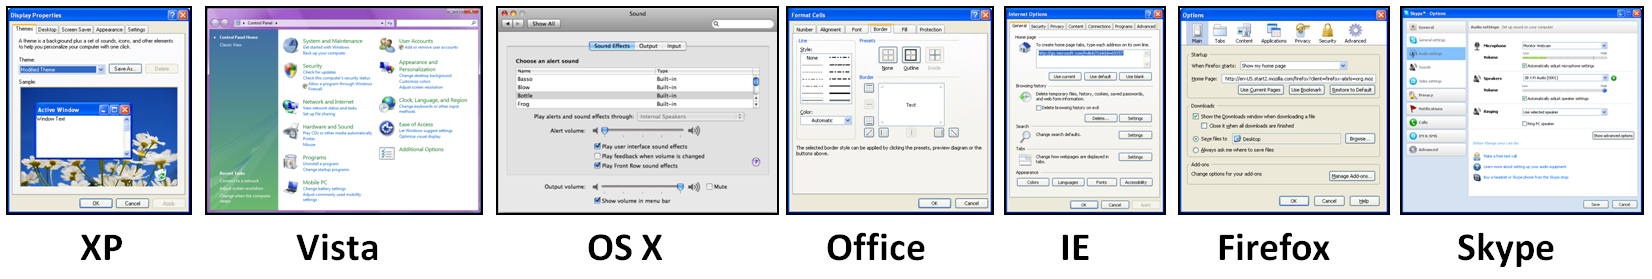
\includegraphics[width=2\columnwidth]{figure/query_examples.png}
\caption{Examples of query images used in screenshot matching
experiments.}
\label{fig:query_examples}
\end{figure*}


\subsection{Compare to keyword search}

In this experiment, we compared the proposed multi-modal search engine
to two keyword search baselines. The first baseline is a commercial
web search engine.  The second baseline is a commercial image search
engine. We were interested in whether users would judge the search
results returned by these three systems differently in terms of
perceived relevancy. We recruited workers from Amazon Mechanical Turk
to perform relevancy judgement.

The comparison is based on 20 query instances (10 XP and 10 Mac
programs). Each query instance was submitted to each of the three
systems. For the two keyword search baselines, we used the words in
the title bar of each program and the name of the operating system as
search terms, for example, mac system preferences. For our system, we
used only the screenshot of the program as the search term. We
collected the top four articles returned by each system and merged
them into a single list of 12. As validation, we added 3 irrelevant
articles and 1 duplicate article to the list. Irrelevant articles were
generated by sampling from the top results returned by the image
search baseline using only one of the search terms, for example, using
the word preferences as the search term for mac system
preferences. Thus, in each assignment, a worker was shown a list of 16
articles and asked to rate the relevancy on a 5-point scale. The list
was randomly shuffled to remove any bias due to ordering.  We only
accepted the ratings given by workers who rated the validation
articles accurately, which was checked by (1) whether irrelevant
articles were rated as irrelevant and (2) whether duplicate articles
were rated consistently. The presence of validation checks
ensure that the optimal strategies for the workers is to
provide answers in an honest manner.

In total, we obtained X unique ratings from Y workers. The 
approval rate was Z. Table X summarizes our findings. 

\subsection{Bilingual search}

In this experiment, we examined the ability of our system to search
across language boundaries. We took screenshots of 15 representative
programs on Mac in five languages (Spanish, French, German,
Chinese, and Korean) and obtained a total of 75 test
images.  We submitted these images to our 
system and retrieved the top 10 matched screenshots. We recorded
the number of correct matches. Table X summarizes
our findings.

\begin{figure*}
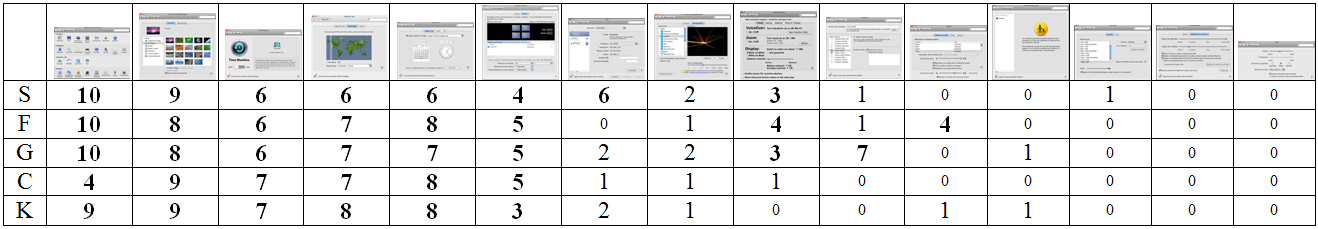
\includegraphics[width=2\columnwidth]{figure/bilingual_search.png}
\caption{Number of correct top 10 matches for 15 programs in five non-English
languages: Spanish (S), French (F), German (G), Chinese (C) and Korean (K).}
\end{figure*}


\section{Discussion}

Keywords can serve two purposes. First, they can specify the
content users wish to see on the returned pages. Second, they can
describe the screenshot to improve the performance of visual
matching. Since the screenshot matching can be done very
accurately, we expect users will very quickly realize that it is
not necessary to repeat the text embedded in the screenshot, since
the visual search will take care of it.


\section{Summary}

\bibliographystyle{plain}
\bibliography{www2010}
\balancecolumns % GM July 2000
% That's all folks!
\end{document}
